\section{Overview}
\label{chapter:TypeShild Overview}
In this section, we present a brief overview on the 
considered adversary model in~\cref{Adversary Model} and depict the 
invariants for calltargets and callsites in~\cref{Invariants for Targets and Callsites}.
Finally, in~\cref{TypeShield Policy Mechanism} we present our function parameter type aware policy and give a formal description of it
by relating it to~\cite{veen:typearmor}, and in~\cref{TypeShild Impact on COOP} we highlight the impact of our policy on COOP.

% \textbf{Adversary Model and Assumptions.}
\subsection{Adversary Model and Assumptions}
\label{Adversary Model}

We largely use the same threat model and the same basic assumptions as described in the TypeArmor 
paper~\cite{veen:typearmor}, meaning that our attacker has read and write access to the data 
sections of the attacked binary.  We also assume that the protected binary does not contain 
self modifying code, handcrafted assembly or any kind of obfuscation. We also consider pages 
to be either writable or executable but not both at the same time. We assume 
that our attacker has the ability to execute a memory corruption to hijack the programs 
control flow and that a solution for backward CFI is in place.

\subsection{Invariants for Calltargets and Callsites}
% \textbf{Invariants for Targets and Callsites.}
\label{Invariants for Targets and Callsites}
Advanced code reuse attacks change the calltargets that are invoked within indirect 
callsites. As standard CFI solutions can hardly restrict these, TypeArmor proposed using two base invariants:
\textit{1)} indirect callsites provide a number of parameters (\textit{i.e.,} possibly overestimated compared to source), and 
\textit{2)} calltargets require a minimum number of parameters (\textit{i.e.,} possibly underestimated compared to source).
The idea is that a callsite might only call functions that do not require more parameters than provided by the callsite. 
To compute the necessary information, TypeArmor uses a modified version of forward liveness analysis for call-targets and 
backward reaching definitions analysis for callsites.

\subsection{\textsc{TypeShield} Policy Mechanism}
\label{TypeShield Policy Mechanism}

\begin{figure}[H]
% \captionsetup{labelformat=empty}
\centering
\resizebox{0.155\textwidth}{!}{
 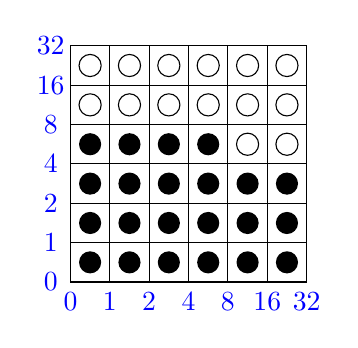
\begin{tikzpicture}
       % labels
%     \foreach \i in {0,...,5}
      \path[blue] (0,-0.25) node{0} (-0.25,0) node{0};
      \path[blue] (1/2,-0.25) node{1} (-0.25,1/2) node{1};
      \path[blue] (2/2,-0.25) node{2} (-0.25,2/2) node{2};
      \path[blue] (3/2,-0.25) node{4} (-0.25,3/2) node{4};
      \path[blue] (4/2,-0.25) node{8} (-0.25,4/2) node{8};
      \path[blue] (5/2,-0.25) node{16} (-0.25,5/2) node{16};
      \path[blue] (6/2,-0.25) node{32} (-0.25,6/2) node{32};
%       \path[blue] (7/2,-0.25) node{64} (-0.25,7/2) node{64};
    % loop over the lattice points
    \foreach \i in {0,...,6}
      \foreach \j in {0,...,6}{
        \draw (\i / 2,\j / 2) rectangle (1,1);
        % check if (\i,\j) > (2,2)
%         \ifnum \i < 3
%           \ifnum \j < 3
%             \fill[red] (\i + 0.25,\j + 0.25) circle(3pt);
%           \fi
%         \fi
      };
      
      \fill (0   + 0.25, 0   + 0.25) circle(4pt);
      \fill (0.5 + 0.25, 0.5 + 0.25) circle(4pt);
      \fill (0 + 0.25, 0.5 + 0.25) circle(4pt);
      \fill (0.5 + 0.25, 0 + 0.25) circle(4pt);
      \fill (0.5 + 0.25, 1 + 0.25) circle(4pt);
      \fill (0 + 0.25, 1 + 0.25) circle(4pt);
      %       \draw [line width=0.5mm, green] (1 + 0.25, 1 + 0.25) circle (6pt);
      
%       \draw (0.5 + 0.25, 3 + 0.25) circle(4pt);
%       \draw (0 + 0.25, 3 + 0.25) circle(4pt);
%       \draw (1 + 0.25, 3 + 0.25) circle(4pt);
%       \draw (1 + 0.75, 3 + 0.25) circle(4pt);
%       \draw (2.25, 3 + 0.25) circle(4pt);
%       \draw (2.75, 3 + 0.25) circle(4pt);
%       \draw (3.25, 3 + 0.25) circle(4pt);
      
      \draw (0.5 + 0.25, 2.5 + 0.25) circle(4pt);
      \draw (0 + 0.25, 2.5 + 0.25) circle(4pt);
      \draw (1 + 0.25, 2.5 + 0.25) circle(4pt);
      \draw (1 + 0.75, 2.5 + 0.25) circle(4pt);
      \draw (2.25, 2.5 + 0.25) circle(4pt);
      \draw (2.75, 2.5 + 0.25) circle(4pt);
%       \draw (3.25, 2.5 + 0.25) circle(4pt);
      
      \draw (0.5 + 0.25, 2 + 0.25) circle(4pt);
      \draw (0 + 0.25, 2 + 0.25) circle(4pt);
      \draw (1 + 0.25, 2 + 0.25) circle(4pt);
      \draw (1 + 0.75, 2 + 0.25) circle(4pt);
      \draw (2.25, 2 + 0.25) circle(4pt);
      \draw (2.75, 2 + 0.25) circle(4pt);
%       \draw (3.25, 2 + 0.25) circle(4pt);
      
      \fill (0.5 + 0.25, 1.5 + 0.25) circle(4pt);
      \fill (0 + 0.25, 1.5 + 0.25) circle(4pt);
      \fill (1 + 0.25, 1.5 + 0.25) circle(4pt);
      \fill (1 + 0.75, 1.5 + 0.25) circle(4pt);
      \draw (2.25, 1.5 + 0.25) circle(4pt);
      \draw (2.75, 1.5 + 0.25) circle(4pt);
%       \draw (3.25, 1.5 + 0.25) circle(4pt);
      
      \fill (1 + 0.25, 1 + 0.25) circle(4pt);
      \fill (1 + 0.75, 1 + 0.25) circle(4pt);
      \fill (2.25, 1 + 0.25) circle(4pt);
      \fill (2.75, 1 + 0.25) circle(4pt);
%       \draw (3.25, 1 + 0.25) circle(4pt);
      
      \fill (1 + 0.25, 0.5 + 0.25) circle(4pt);
      \fill (1 + 0.75, 0.5 + 0.25) circle(4pt);
      \fill (2.25, 0.5 + 0.25) circle(4pt);
      \fill (2.75, 0.5 + 0.25) circle(4pt);
%       \fill (3.25, 0.5 + 0.25) circle(4pt);
      
      \fill (1 + 0.25, 0 + 0.25) circle(4pt);
      \fill (1 + 0.75, 0 + 0.25) circle(4pt);
      \fill (2.25, 0 + 0.25) circle(4pt);
      \fill (2.75, 0 + 0.25) circle(4pt);
%       \fill (3.25, 0 + 0.25) circle(4pt);
  \end{tikzpicture}}
\textbf{$\wedge$}
\hspace{.01cm}% NO SPACE!
\resizebox{0.155\textwidth}{!}{
 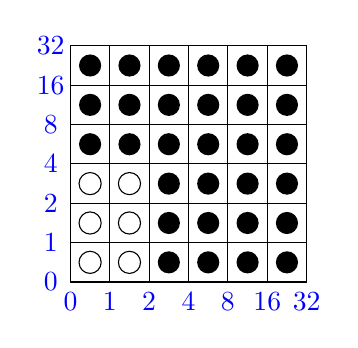
\begin{tikzpicture}
       % labels
%     \foreach \i in {0,...,5}
      \path[blue] (0,-0.25) node{0} (-0.25,0) node{0};
      \path[blue] (1/2,-0.25) node{1} (-0.25,1/2) node{1};
      \path[blue] (2/2,-0.25) node{2} (-0.25,2/2) node{2};
      \path[blue] (3/2,-0.25) node{4} (-0.25,3/2) node{4};
      \path[blue] (4/2,-0.25) node{8} (-0.25,4/2) node{8};
      \path[blue] (5/2,-0.25) node{16} (-0.25,5/2) node{16};
      \path[blue] (6/2,-0.25) node{32} (-0.25,6/2) node{32};
%       \path[blue] (7/2,-0.25) node{64} (-0.25,7/2) node{64};
    % loop over the lattice points
    \foreach \i in {0,...,6}
      \foreach \j in {0,...,6}{
        \draw (\i / 2,\j / 2) rectangle (1,1);
        % check if (\i,\j) > (2,2)
%         \ifnum \i < 3
%           \ifnum \j < 3
%             \fill[red] (\i + 0.25,\j + 0.25) circle(3pt);
%           \fi
%         \fi
      };
      
      \draw (0   + 0.25, 0   + 0.25) circle(4pt);
      \draw (0.5 + 0.25, 0.5 + 0.25) circle(4pt);
      \draw (0 + 0.25, 0.5 + 0.25) circle(4pt);
      \draw (0.5 + 0.25, 0 + 0.25) circle(4pt);
      \draw (0.5 + 0.25, 1 + 0.25) circle(4pt);
      \draw (0 + 0.25, 1 + 0.25) circle(4pt);
      
%       \fill (0.5 + 0.25, 3 + 0.25) circle(4pt);
%       \fill (0 + 0.25, 3 + 0.25) circle(4pt);
%       \fill (1 + 0.25, 3 + 0.25) circle(4pt);
%       \fill (1 + 0.75, 3 + 0.25) circle(4pt);
%       \fill (2.25, 3 + 0.25) circle(4pt);
%       \fill (2.75, 3 + 0.25) circle(4pt);
%       \fill (3.25, 3 + 0.25) circle(4pt);
      
      \fill (0.5 + 0.25, 2.5 + 0.25) circle(4pt);
      \fill (0 + 0.25, 2.5 + 0.25) circle(4pt);
      \fill (1 + 0.25, 2.5 + 0.25) circle(4pt);
      \fill (1 + 0.75, 2.5 + 0.25) circle(4pt);
      \fill (2.25, 2.5 + 0.25) circle(4pt);
      \fill (2.75, 2.5 + 0.25) circle(4pt);
%       \fill (3.25, 2.5 + 0.25) circle(4pt);
      
      \fill (0.5 + 0.25, 2 + 0.25) circle(4pt);
      \fill (0 + 0.25, 2 + 0.25) circle(4pt);
      \fill (1 + 0.25, 2 + 0.25) circle(4pt);
      \fill (1 + 0.75, 2 + 0.25) circle(4pt);
      \fill (2.25, 2 + 0.25) circle(4pt);
      \fill (2.75, 2 + 0.25) circle(4pt);
%       \fill (3.25, 2 + 0.25) circle(4pt);
      
      \fill (0.5 + 0.25, 1.5 + 0.25) circle(4pt);
      \fill (0 + 0.25, 1.5 + 0.25) circle(4pt);
      \fill (1 + 0.25, 1.5 + 0.25) circle(4pt);
      \fill (1 + 0.75, 1.5 + 0.25) circle(4pt);
      \fill (2.25, 1.5 + 0.25) circle(4pt);
      \fill (2.75, 1.5 + 0.25) circle(4pt);
%       \fill (3.25, 1.5 + 0.25) circle(4pt);
      
      \fill (1 + 0.25, 1 + 0.25) circle(4pt);
      \fill (1 + 0.75, 1 + 0.25) circle(4pt);
      \fill (2.25, 1 + 0.25) circle(4pt);
      \fill (2.75, 1 + 0.25) circle(4pt);
%       \fill (3.25, 1 + 0.25) circle(4pt);
      
      \fill (1 + 0.25, 0.5 + 0.25) circle(4pt);
      \fill (1 + 0.75, 0.5 + 0.25) circle(4pt);
      \fill (2.25, 0.5 + 0.25) circle(4pt);
      \fill (2.75, 0.5 + 0.25) circle(4pt);
%       \fill (3.25, 0.5 + 0.25) circle(4pt);
      
      \fill (1 + 0.25, 0 + 0.25) circle(4pt);
      \fill (1 + 0.75, 0 + 0.25) circle(4pt);
      \fill (2.25, 0 + 0.25) circle(4pt);
      \fill (2.75, 0 + 0.25) circle(4pt);
%       \fill (3.25, 0 + 0.25) circle(4pt);
      
  \end{tikzpicture}}
\textbf{$=$}
\hspace{.01cm}% NO SPACE!
\resizebox{0.155\textwidth}{!}{
 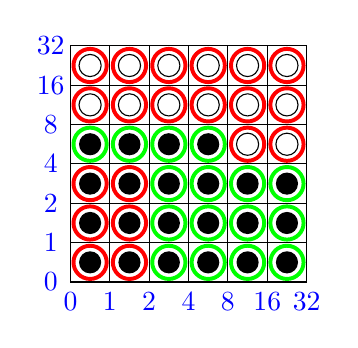
\begin{tikzpicture}
    % labels
%     \foreach \i in {0,...,5}
      \path[blue] (0,-0.25) node{0} (-0.25,0) node{0};
      \path[blue] (1/2,-0.25) node{1} (-0.25,1/2) node{1};
      \path[blue] (2/2,-0.25) node{2} (-0.25,2/2) node{2};
      \path[blue] (3/2,-0.25) node{4} (-0.25,3/2) node{4};
      \path[blue] (4/2,-0.25) node{8} (-0.25,4/2) node{8};
      \path[blue] (5/2,-0.25) node{16} (-0.25,5/2) node{16};
      \path[blue] (6/2,-0.25) node{32} (-0.25,6/2) node{32};
%       \path[blue] (7/2,-0.25) node{64} (-0.25,7/2) node{64};
    % loop over the lattice points
    \foreach \i in {0,...,6}
      \foreach \j in {0,...,6}{
        \draw (\i / 2,\j / 2) rectangle (1,1);
        % check if (\i,\j) > (2,2)
%         \ifnum \i < 3
%           \ifnum \j < 3
%             \fill[red] (\i + 0.25,\j + 0.25) circle(3pt);
%           \fi
%         \fi
      };
      
      \fill (0   + 0.25, 0   + 0.25) circle(4pt);
      \draw [line width=0.5mm, red] (0   + 0.25, 0   + 0.25) circle (6pt);
      \fill (0.5 + 0.25, 0.5 + 0.25) circle(4pt);
      \draw [line width=0.5mm, red] (0.5 + 0.25, 0.5 + 0.25) circle (6pt);
      \fill (0 + 0.25, 0.5 + 0.25) circle(4pt);
      \draw [line width=0.5mm, red] (0 + 0.25, 0.5 + 0.25) circle (6pt);
      \fill (0.5 + 0.25, 0 + 0.25) circle(4pt);
      \draw [line width=0.5mm, red] (0.5 + 0.25, 0 + 0.25) circle (6pt);
      \fill (0.5 + 0.25, 1 + 0.25) circle(4pt);
      \draw [line width=0.5mm, red] (0.5 + 0.25, 1 + 0.25) circle (6pt);
      \fill (0 + 0.25, 1 + 0.25) circle(4pt);
      \draw [line width=0.5mm, red] (0 + 0.25, 1 + 0.25) circle (6pt);
      
%       \draw (0.5 + 0.25, 3 + 0.25) circle(4pt);
%       \draw [line width=0.5mm, red] (0.5 + 0.25, 3 + 0.25) circle (6pt);
%       \draw (0 + 0.25, 3 + 0.25) circle(4pt);
%       \draw [line width=0.5mm, red] (0 + 0.25, 3 + 0.25) circle (6pt);
%       \draw (1 + 0.25, 3 + 0.25) circle(4pt);
%       \draw [line width=0.5mm, red] (1 + 0.25, 3 + 0.25) circle (6pt);
%       \draw (1 + 0.75, 3 + 0.25) circle(4pt);
%       \draw [line width=0.5mm, red] (1 + 0.75, 3 + 0.25) circle (6pt);
%       \draw (2.25, 3 + 0.25) circle(4pt);
%       \draw [line width=0.5mm, red] (2.25, 3 + 0.25) circle (6pt);
%       \draw (2.75, 3 + 0.25) circle(4pt);
%       \draw [line width=0.5mm, red] (2.75, 3 + 0.25) circle (6pt);
%       \draw (3.25, 3 + 0.25) circle(4pt);
%       \draw [line width=0.5mm, red] (3.25, 3 + 0.25) circle (6pt);
      
      \draw (0.5 + 0.25, 2.5 + 0.25) circle(4pt);
      \draw [line width=0.5mm, red] (0.5 + 0.25, 2.5 + 0.25) circle (6pt);
      \draw (0 + 0.25, 2.5 + 0.25) circle(4pt);
      \draw [line width=0.5mm, red] (0 + 0.25, 2.5 + 0.25) circle (6pt);
      \draw (1 + 0.25, 2.5 + 0.25) circle(4pt);
      \draw [line width=0.5mm, red] (1 + 0.25, 2.5 + 0.25) circle (6pt);
      \draw (1 + 0.75, 2.5 + 0.25) circle(4pt);
      \draw [line width=0.5mm, red] (1 + 0.75, 2.5 + 0.25) circle (6pt);
      \draw (2.25, 2.5 + 0.25) circle(4pt);
      \draw [line width=0.5mm, red] (2.25, 2.5 + 0.25) circle (6pt);
      \draw (2.75, 2.5 + 0.25) circle(4pt);
      \draw [line width=0.5mm, red] (2.75, 2.5 + 0.25) circle (6pt);
%       \draw (3.25, 2.5 + 0.25) circle(4pt);
%       \draw [line width=0.5mm, red] (3.25, 2.5 + 0.25) circle (6pt);
      
      \draw (0.5 + 0.25, 2 + 0.25) circle(4pt);
      \draw [line width=0.5mm, red] (0.5 + 0.25, 2 + 0.25) circle (6pt);
      \draw (0 + 0.25, 2 + 0.25) circle(4pt);
      \draw [line width=0.5mm, red] (0 + 0.25, 2 + 0.25) circle (6pt);
      \draw (1 + 0.25, 2 + 0.25) circle(4pt);
      \draw [line width=0.5mm, red] (1 + 0.25, 2 + 0.25) circle (6pt);
      \draw (1 + 0.75, 2 + 0.25) circle(4pt);
      \draw [line width=0.5mm, red] (1 + 0.75, 2 + 0.25) circle (6pt);
      \draw (2.25, 2 + 0.25) circle(4pt);
      \draw [line width=0.5mm, red] (2.25, 2 + 0.25) circle (6pt);
      \draw (2.75, 2 + 0.25) circle(4pt);
      \draw [line width=0.5mm, red] (2.75, 2 + 0.25) circle (6pt);
%       \draw (3.25, 2 + 0.25) circle(4pt);
%       \draw [line width=0.5mm, red] (3.25, 2 + 0.25) circle (6pt);
      
      \fill (0.5 + 0.25, 1.5 + 0.25) circle(4pt);
      \draw [line width=0.5mm, green] (0.5 + 0.25, 1.5 + 0.25) circle (6pt);
      \fill (0 + 0.25, 1.5 + 0.25) circle(4pt);
      \draw [line width=0.5mm, green] (0 + 0.25, 1.5 + 0.25) circle (6pt);
      \fill (1 + 0.25, 1.5 + 0.25) circle(4pt);
      \draw [line width=0.5mm, green] (1 + 0.25, 1.5 + 0.25) circle (6pt);
      \fill (1 + 0.75, 1.5 + 0.25) circle(4pt);
      \draw [line width=0.5mm, green] (1 + 0.75, 1.5 + 0.25) circle (6pt);
      \draw (2.25, 1.5 + 0.25) circle(4pt);
      \draw [line width=0.5mm, red] (2.25, 1.5 + 0.25) circle (6pt);
      \draw (2.75, 1.5 + 0.25) circle(4pt);
      \draw [line width=0.5mm, red] (2.75, 1.5 + 0.25) circle (6pt);
%       \draw (3.25, 1.5 + 0.25) circle(4pt);
%       \draw [line width=0.5mm, red] (3.25, 1.5 + 0.25) circle (6pt);
      
      \fill (1 + 0.25, 1 + 0.25) circle(4pt);
      \draw [line width=0.5mm, green] (1 + 0.25, 1 + 0.25) circle (6pt);
      \fill (1 + 0.75, 1 + 0.25) circle(4pt);
      \draw [line width=0.5mm, green] (1 + 0.75, 1 + 0.25) circle (6pt);
      
      \fill (2.25, 1 + 0.25) circle(4pt);
      \draw [line width=0.5mm, green] (2.25, 1 + 0.25) circle (6pt);
      \fill (2.75, 1 + 0.25) circle(4pt);
      \draw [line width=0.5mm, green] (2.75, 1 + 0.25) circle (6pt);
%       \draw (3.25, 1 + 0.25) circle(4pt);
%       \draw [line width=0.5mm, red] (3.25, 1 + 0.25) circle (6pt);
      
      \fill (1 + 0.25, 0.5 + 0.25) circle(4pt);
      \draw [line width=0.5mm, green] (1 + 0.25, 0.5 + 0.25) circle (6pt);
      \fill (1 + 0.75, 0.5 + 0.25) circle(4pt);
      \draw [line width=0.5mm, green] (1 + 0.75, 0.5 + 0.25) circle (6pt);
      \fill (2.25, 0.5 + 0.25) circle(4pt);
      \draw [line width=0.5mm, green] (2.25, 0.5 + 0.25) circle (6pt);
      \fill (2.75, 0.5 + 0.25) circle(4pt);
      \draw [line width=0.5mm, green] (2.75, 0.5 + 0.25) circle (6pt);
%       \draw (3.25, 0.5 + 0.25) circle(4pt);
%       \draw [line width=0.5mm, red] (3.25, 0.5 + 0.25) circle (6pt);
      
      \fill (1 + 0.25, 0 + 0.25) circle(4pt);
      \draw [line width=0.5mm, green] (1 + 0.25, 0 + 0.25) circle (6pt);
      \fill (1 + 0.75, 0 + 0.25) circle(4pt);
      \draw [line width=0.5mm, green] (1 + 0.75, 0 + 0.25) circle (6pt);
      \fill (2.25, 0 + 0.25) circle(4pt);
      \draw [line width=0.5mm, green] (2.25, 0 + 0.25) circle (6pt);
      \fill (2.75, 0 + 0.25) circle(4pt);
      \draw [line width=0.5mm, green] (2.75, 0 + 0.25) circle (6pt);
%       \draw (3.25, 0 + 0.25) circle(4pt);
%       \draw [line width=0.5mm, red] (3.25, 0 + 0.25) circle (6pt);
\end{tikzpicture}}
\caption{Type and parameter count policy. Note that our type policy performs an $\wedge$ operation
between each entry in the first and second matrices. If at least one match is present on all of the columns of the 
third matrix than the indirect call transfer will be allowed by our policy, otherwise not. In this given situation
the indirect call transfer will be allowed.}
\label{Type and parameter count policy.}
\end{figure}

Figure~\ref{Type and parameter count policy.} depicts the behavior of our type based policy
when the callsite provides 6 parameters $pcs1, ..., pcs6$ having following bit 
wideness \textit{pcs}1:4-byte, \textit{pcs}2:4-bye, \textit{pcs}3-4-byte, \textit{pcs}4:4-byte, \textit{pcs}5-2-byte, 
\textit{pcs}6:2-byte, and the calltarget is expecting 6 parameters $pct1, ..., pcs6$ having following bit 
wideness \textit{pct}1:4-byte, \textit{pct}2:4-bye, \textit{pct}3:0-byte, \textit{pct}4:0-byte, \textit{pct}5:0-byte, 
\textit{pct}6:0-byte of the expected parameters. 
\textsc{TypeShield}'s type policy is: 
\begin{multline}
Let \ A \ be \ a \ calltarget \ ct_{A} \ and \ cs_{B} \ be \ a \ callsite \ than: 
\\ ct_{A} \subseteq cs_{B} \iff \forall i \exists [1, 6], 
wideness(paramter(A)[i]) \leq \\ wideness(paramter(B)[i]).
\end{multline}

Whereas the policy of TypeArmor is: 
\begin{multline}
Let \ A \ be \ a \ calltarget \ ct_{A} \ and \ cs_{B} \ be \ a \ callsite \ than: 
\\ ct_{A} \subseteq cs_{B} \iff \forall i \exists [1, 6], 
count(paramter(A)) \leq \\ count(paramter(B)).
\end{multline}


\subsection{\textsc{TypeShield} Impact on COOP}
% \textbf{\textsc{TypeShield} Impact on COOP.}
\label{TypeShild Impact on COOP}
\begin{figure}[h!]
\centering
\resizebox{0.45\textwidth}{!}{
\begin{tikzpicture}

\draw[thick] (0,-3) [blue] rectangle node[anchor=center]  (0)  {\LARGE{$\bot:$ | 0 | 0 | 0 | 0 | 0 | 0 |}}   (6,-4);

\draw[thick] (0,0) rectangle node[anchor=center]  (320)  {\LARGE{| 32 | 0 | 0 | 0 | 0 | 0 |}}  (6,-1);

\draw[thick] (7,1.5) rectangle node[anchor=center]  (640)  {\LARGE{| 64 | 0 | 0 | 0 | 0 | 0 |}}  (13,0.5);

\draw[thick] (0,2) rectangle node[anchor=center]  (3232) {\LARGE{| 32 | 32 | 0 | 0 | 0 | 0 |}} (6,3);

\draw[thick] (7,5) rectangle node[anchor=center]  (6432) {\LARGE{| 64 | 32 | 0 | 0 | 0 | 0 |}} (13,6);

\draw[thick] (-1,5) rectangle node[anchor=center] (3264) {\LARGE{| 32 | 64 | 0 | 0 | 0 | 0 |}} (-7,6);

\draw[thick] (0,8) [blue] rectangle node[anchor=center]  (6464) {\LARGE{$\top:$ |64|64|64|64|64|64|}} (6,9);

  \draw[draw, -triangle 45, thick] (3264.north) -- (6464.south);
  \draw[draw, -triangle 45, thick] (6432.north) -- (6464.south);
  \draw[draw, -triangle 45, thick] (3232.north) -- (3264.south);
  \draw[draw, -triangle 45, thick] (3232.north) -- (6432.south);
  \draw[draw, -triangle 45, thick] (640.north) -- (6432.south);
  \draw[draw, -triangle 45, thick] (320.north) -- (3232.south);
  \draw[draw, -triangle 45, thick] (320.north) -- (640.south);
  \draw[draw, -triangle 45, thick] (0.north) -- (320.south);
  
\end{tikzpicture}
}
\caption{Parameter register wideness based lattice using 64-bit, 32-bit and 0-bit parameter wideness with six 
function parameters. Note that $\top$ and $\bot$ represents the top and bottom element of the lattice, respectively.
An arrow (\textit{i.e.,} in total 8) represents an indirect control flow transfer from a callsite to a calltarget. Note that~\cite{veen:typearmor}
would allow all 8 illegal control flow transfers and that \textsc{TypeSchield} would forbid all of them.}
\label{fig:lattice3264}
\end{figure}
Figure~\ref{fig:lattice3264} represents the a sub-part of the total indirect transfers space in any given C/C++ program. 
In case a CFI policy schema is based only on parameter count it is possible that any callsite can use any call-target as long as the number of 
parameter requirement is fulfilled, even if the parameter types do not match (\textit{i.e.,} imagine 8-bit values provided by the callsite
but 64-bit values required by the calltarget). Such a parameter type \textit{blind} policy would allow any call transfer inside the lattice
space presented in Figure~\ref{fig:lattice3264} and as such the calltarget set per callsite would be too permissive.

In order to effectively deal with this situation we extend the CFI classification schema to the function parameter types by introducing the following 
policy rules: \textit{1)} indirect callsites provide a maximum wideness to each parameter, and
\textit{2)} calltargets require a minimum wideness for each parameter. Note that for both rules the minimum and maximum wideness for each function 
parameter is possibly underestimated compared to the source code of the program with which we also compare in \cref{chapter:Evaluation}.
Note, that the provision must be no lower than the requirement w.r.t. the number of parameters. 
Finally, our approach is more fine-grained by considering parameter wideness and as such the addressable 
calltarget lattice space is considerably reduced.



% The result is that we split the buckets of TypeArmor up into smaller ones as shown 
% in the limited example depicted in Figure \ref{fig:lattice3264}.
% There we can see that while in a parameter-count oriented schema a callsite classified as (32,32) would be able to 
% call functions classified as (64,0), however in our parameter wideness oriented schema that is not possible.
